\section{Research \& development}
This department of AllSpark is involved in all the activities related to
improve and realize new products as research projects. This sector is
considered a relevant one in the organization business, in fact this sector
has the aim to bring innovation and distinguish our products among the
competitors.

An important feature of this area is the strong collaboration between
AllSpark and various foundation operating in the OpenSource community
environment.
These collaborations are based on active support of AllSpark during the
development of their project. The support AllSpark is offering id mainly
focused on patching and bugfixing, but can be expanded to founding or other
ways of collaboration.

\subsection{Search Sector}
The main aim of this process is to look for a research sector in which
instantiate a new r\&d project. Mainly is devolved to handle security
related sectors, due to the high risks and frequent changes always present
in this area.

The process involves an analysis of the newest studies on security issues
and menaces in IT systems, its results are useful for performing an
investigation about possible vulnerabilities in AllSparks products. Is
important to notice that other than check a single product is important to
consider the whole offer of AllSpark, looking for possible problems which
are not covered by the existing products but still in the scope of AllSpark
activity.

Image \ref{2img:sector} describes this process in its details.

\begin{figure}[!ht]
\begin{centering}
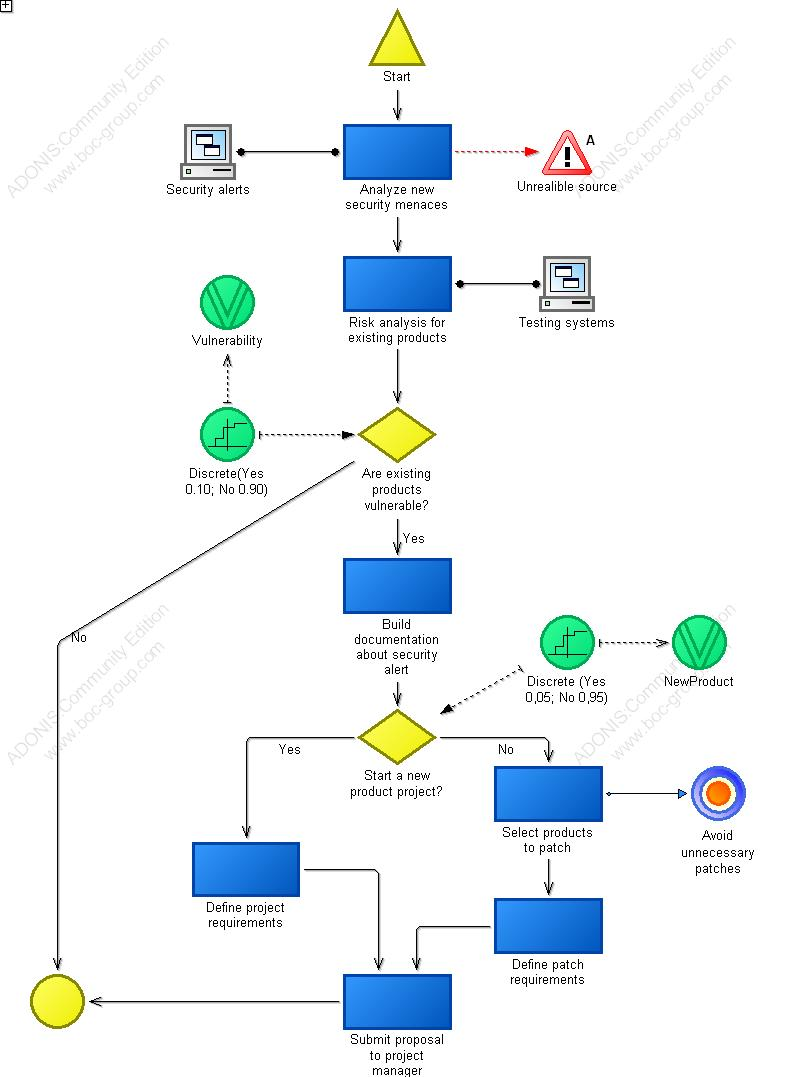
\includegraphics[scale=0.50]{assign2/adonis/imgs/sector.jpg}
\caption{Search sector AllSpark process}
\label{2img:sector}
\end{centering}
\end{figure}

\subsubsection{Path Analysis}
The result of the path analysis, shows that the most probable results is
that there are no such menaces which can trigger the starting of a new
research project.

\begin{table}[ht!]
\centering
\begin{tabular}{|l|l|l|l|l|}
\hline
Path&Probability&Execution time&Cycle time&Costs\\
\hline
1&0,899000&00:000:02:30:00&00:000:02:30:00&6,000000\\
\hline
2&0,092000&00:000:03:07:00&00:000:03:07:00&7,400000\\
\hline
3&0,009000&00:000:03:02:00&00:000:03:02:00&7,700000\\
\hline
\end{tabular}
\end{table}

\begin{alltt}
Probability:   89,9000%
Execution time:  00:000:02:30:00
Waiting time:  00:000:00:00:00
Resting time:  00:000:00:00:00
Transport time:  00:000:00:00:00
Cycle time:  00:000:02:30:00
Costs:  6,000000

Search sector 0.3 (Business process model)
========================================
Process start: Start
Activity: Analyze new security menaces
Activity: Risk analysis for existing products
Decision: Are existing products vulnerable? --> Vulnerability = 'No'
End: End
\end{alltt}

\subsubsection{Capacity Analysis}
Table \ref{2tab:sector} depicts the capacity analysis for the process of
searching a sector in which start a new research project.

\begin{landscape}
\centering
\begin{table}
{\tiny
\begin{tabular}{|l|l|l|l|l|l|l|}
Business process&Activity&Performer&Number&Execution time&Cycle
time&Costs\\
\hline
Search sector 0.3&&&&00:000:02:33:42&00:000:02:33:42&6,143200\\
\hline
&Analyze new security menaces &&1,000000&00:000:00:30:00&&1,000000\\
\hline
&&Area Manager &1,000000&00:000:00:30:00&&1,000000\\
\hline
&Risk analysis for existing products &&1,000000&00:000:02:00:00&&5,000000\\
\hline
&&Area Manager &1,000000&00:000:02:00:00&&5,000000\\
\hline
&Build documentation about security alert &&0,101000&00:000:00:02:01&&0,050500\\
\hline
&&Area Manager &0,101000&00:000:00:02:01&&0,050500\\
\hline
&Select products to patch &&0,095000&00:000:00:00:29&&0,047500\\
\hline
&&Programmer &0,049000&00:000:00:00:15&&0,024500\\
\hline
&&Analyst &0,046000&00:000:00:00:14&&0,023000\\
\hline
&Define project requirements &&0,006000&00:000:00:00:04&&0,006000\\
\hline
&&Area Manager &0,006000&00:000:00:00:04&&0,006000\\
\hline
&Define patch requirements &&0,095000&00:000:00:00:57&&0,019000\\
\hline
&&Area Manager &0,095000&00:000:00:00:57&&0,019000\\
\hline
&Submit proposal to project manager &&0,101000&00:000:00:00:12&&0,020200\\
\hline
&&Area Manager &0,101000&00:000:00:00:12&&0,020200\\
\hline
Total&&&&00:000:02:33:42&&6,143200\\
\hline
\end{tabular}
}
\caption{Capacity analysis for the process of selecting a sector for a new project} 
\label{2tab:sector}
\end{table}
\end{landscape}





\subsection{Search Updates}
In the IT environment trends and actual needs are often changing, is
therefore necessary to track these development in order to be prepared and
offer always updated products which can actually encounter costumer's
needs.

The aim of this process is to analyze the evolving market data and monitor
the trends in products usage. In this way AllSpark can retrieve a reliable
picture of the market trends.
The results of this analysis can be used to check whether there is the need
for developing a new product, or if is sufficient to add new features and
extensions to an existing one.

This process is depicted in image \ref{2img:search_upd}.

\begin{figure}[!ht]
\begin{centering}
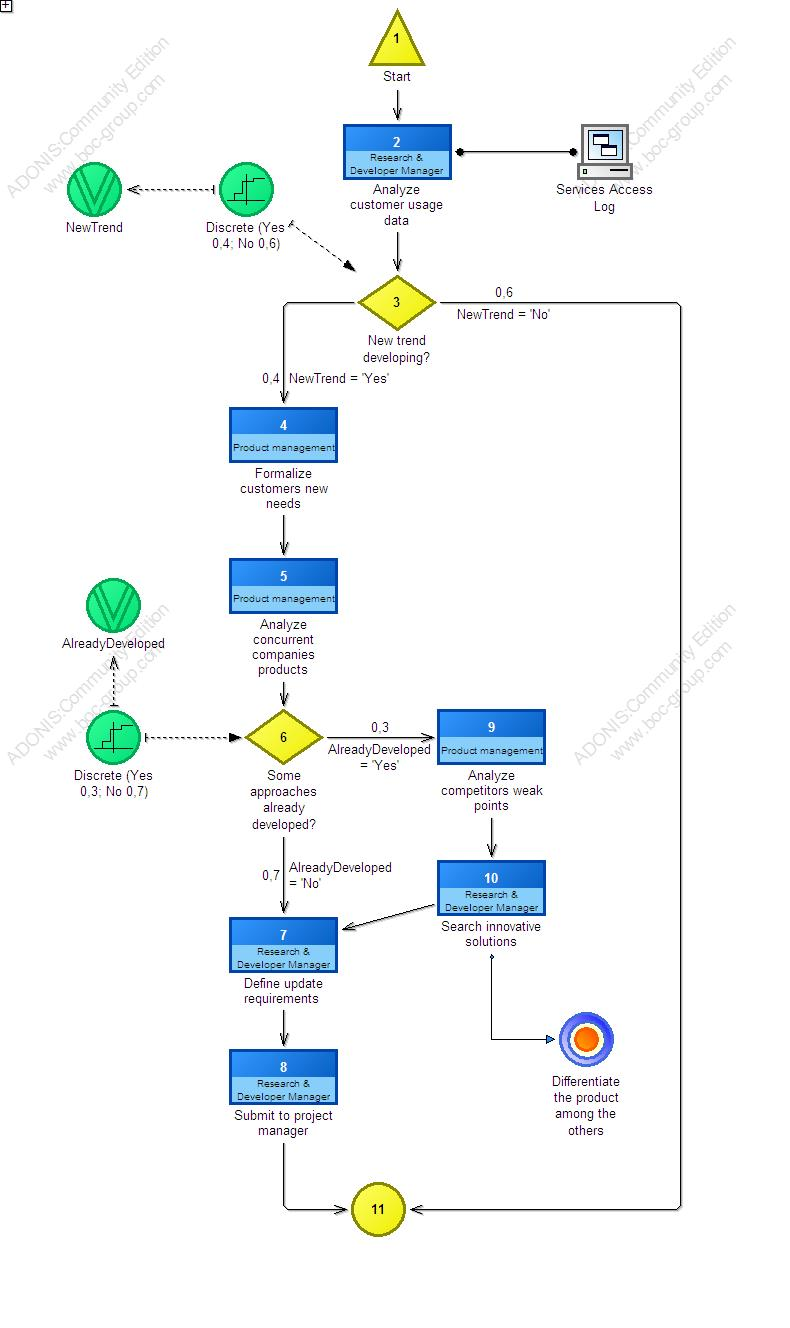
\includegraphics[scale=0.50]{assign2/adonis/imgs/search_upd.jpg}
\caption{Update searching process}
\label{2img:search_upd}
\end{centering}
\end{figure}

\subsubsection{Path Analysis}
The analysis of the possible paths shows that the evolution of the customer
trends, not always leads to the developing of new products.

\begin{table}[ht!]
\centering
\begin{tabular}{|l|l|l|l|l|}
\hline
Path&Probability&Execution time&Cycle time&Costs\\
\hline
1&0,601000&00:000:00:10:00&00:000:00:10:00&2,000000\\
\hline
2&0,264000&00:000:01:52:00&00:000:01:52:00&67,200000\\
\hline
3&0,135000&00:000:03:37:00&00:000:03:37:00&217,200000\\
\hline
\end{tabular}
\end{table}

\begin{alltt}
Probability:   60,1000%
Execution time:  00:000:00:10:00
Waiting time:  00:000:00:00:00
Resting time:  00:000:00:00:00
Transport time:  00:000:00:00:00
Cycle time:  00:000:00:10:00
Costs:  2,000000

Search Updates 0.3 (Business process model)
========================================
Process start: Start
Activity: Analyze customer usage data
Decision: New trend developing? --> NewTrend = 'No'
End: End-44324
\end{alltt}

\subsubsection{Capacity Analysis}
Table \ref{2tab:updates} depicts the results of the capacity analysis of
this process.
\begin{landscape}
\centering
\begin{table}
{\tiny
\begin{tabular}{|l|l|l|l|l|l|l|}
Business process&Activity&Performer&Number&Execution time&Cycle
time&Costs\\
\hline
Search Updates 0.3&&&&00:000:01:03:53&00:000:01:03:53&45,812400\\
\hline
&Analyze customer usage data &&1,000000&00:000:00:10:00&&2,000000\\
\hline
&&Area Manager &1,000000&00:000:00:10:00&&2,000000\\
\hline
&Formalize customers new needs &&0,412000&00:000:00:08:14&&4,120000\\
\hline
&&Programmer &0,204000&00:000:00:04:05&&2,040000\\
\hline
&&Analyst &0,208000&00:000:00:04:10&&2,080000\\
\hline
&Analyze concurrent companies products &&0,412000&00:000:00:24:43&&20,600000\\
\hline
&&Programmer &0,206000&00:000:00:12:22&&10,300000\\
\hline
&&Analyst &0,206000&00:000:00:12:22&&10,300000\\
\hline
&Search innovative solutions &&0,113000&00:000:00:06:47&&11,300000\\
\hline
&&Area Manager &0,113000&00:000:00:06:47&&11,300000\\
\hline
&Define update requirements  &&0,412000&00:000:00:08:14&&2,060000\\
\hline
&&Area Manager &0,412000&00:000:00:08:14&&2,060000\\
\hline
&Analyze competitors weak points &&0,113000&00:000:00:05:05&&5,650000\\
\hline
&&Programmer &0,067000&00:000:00:03:01&&3,350000\\
\hline
&&Analyst &0,046000&00:000:00:02:04&&2,300000\\
\hline
&Submit to project manager &&0,412000&00:000:00:00:49&&0,082400\\
\hline
&&Area Manager &0,412000&00:000:00:00:49&&0,082400\\
\hline
Total&&&&00:000:01:03:53&&45,812400\\
\hline
\end{tabular}
}
\caption{Capacity analysis for the process of searching updates for a
product} 
\label{2tab:updates}
\end{table}
\end{landscape}



\subsection{Search bug}
This process describes how AllSpark handles with failures in its own
research project. In this process, in fact, developers are involved in
finding and fixing errors in existing projects.

In this process the main attention is focused on performing smart tests in
order to find and resolve the problems. One important thing is to notice
the difference between the two kinds of test which are going to be
performed.
In fact, after a first analysis of the code, is necessary to develop a
series of test cases which provides a wide coverage over the possible
different behaviour of the system. When the bug is located and a patch is
prepared, a sharper approach is needed, in order to test that particular
portion of the system. The process used in AllSpark to deal with bug
problems in research project is described in figure \ref{2img:search_bug}.

\begin{figure}[!ht]
\begin{centering}
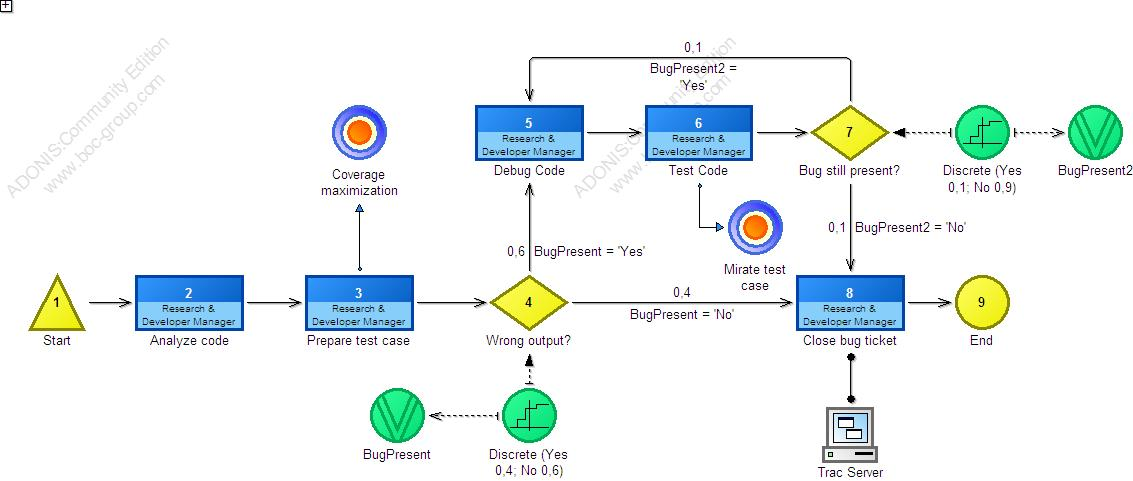
\includegraphics[scale=0.50, angle=90]{assign2/adonis/imgs/debug.jpg}
\caption{AllSparks debug process for Research project}
\label{2img:search_bug}
\end{centering}
\end{figure}

\subsubsection{Path Analysis}
The most probable path for this process determines the normal condition in
which no bugs are found in the analyzed application.
\begin{table}[ht!]
\centering
\begin{tabular}{|l|l|l|l|l|}
\hline
Path&Probability&Execution time&Cycle time&Costs\\
\hline
1&0,624000&00:000:01:15:00&00:000:01:15:00&11,400000\\
\hline
2&0,333000&00:001:01:45:00&00:001:01:45:00&221,400000\\
\hline
3&0,039000&00:002:02:15:00&00:002:02:15:00&431,400000\\
\hline
4&0,004000&00:003:02:45:00&00:003:02:45:00&641,400000\\
\hline
\end{tabular}
\end{table}

\begin{alltt}
Probability:   62,4000%
Execution time:  00:000:01:15:00
Waiting time:  00:000:00:00:00
Resting time:  00:000:00:00:00
Transport time:  00:000:00:00:00
Cycle time:  00:000:01:15:00
Costs:  11,400000

Search bug 0.3 (Business process model)
========================================
Process start: Start
Activity: Analyze code
Activity: Prepare test case
Decision: Wrong output? --> BugPresent = 'No'
Activity: Close bug ticket
End: End
\end{alltt}

\subsubsection{Capacity Analysis}
Table \ref{2tab:debug} is the result of the capacity analysis of this
process
\begin{landscape}
\centering
\begin{table}
{\tiny
\begin{tabular}{|l|l|l|l|l|l|l|}
Business process&Activity&Performer&Number&Execution time&Cycle
time&Costs\\
\hline
Search bug 0.3&&&&00:000:05:37:43&00:000:05:37:43&98,970000\\
\hline
&Analyze code &&1,000000&00:000:00:40:00&&1,000000\\
\hline
&&Area Manager &1,000000&00:000:00:40:00&&1,000000\\
\hline
&Prepare test case &&1,000000&00:000:00:30:00&&10,000000\\
\hline
&&Area Manager &1,000000&00:000:00:30:00&&10,000000\\
\hline
&Debug Code &&0,417000&00:000:04:10:12&&83,400000\\
\hline
&&Area Manager &0,417000&00:000:04:10:12&&83,400000\\
\hline
&Test Code &&0,417000&00:000:00:12:31&&4,170000\\
\hline
&&Area Manager &0,417000&00:000:00:12:31&&4,170000\\
\hline
&Close bug ticket &&1,000000&00:000:00:05:00&&0,400000\\
\hline
&&Area Manager &1,000000&00:000:00:05:00&&0,400000\\
\hline
Total&&&&00:000:05:37:43&&98,970000\\
\hline
\end{tabular}
}
\caption{Capacity analysis for the process of debugging a research project} 
\label{2tab:debug}
\end{table}
\end{landscape}



\subsection{Foundation Cooperation}
As said before, one of the aim of AllSpark is be engaged in an active
collaboration with the entities working in the OpenSource field. The
benefit of this collaboration is to be evaluated in an economic sense from
one side, and from a reputation point of view form the other.

For the foundations could be an opportunity to gain renown if AllSpark
products integrate their solutions. Apart from this the collaboration can
be based on financial founding or, as in the case of the research project,
on active collaboration on software developing.

This collaboration extends to bugfixing and patching the software, not to
strategic decisions on the direction of the development, this to preserve
the independence of the Foundation in its business.

The project of the patching activities for software not developed by
AllSpark, but by an OpenSource Foundation is described by figure
\ref{2img:found_coop}

\begin{figure}[!ht]
\begin{centering}
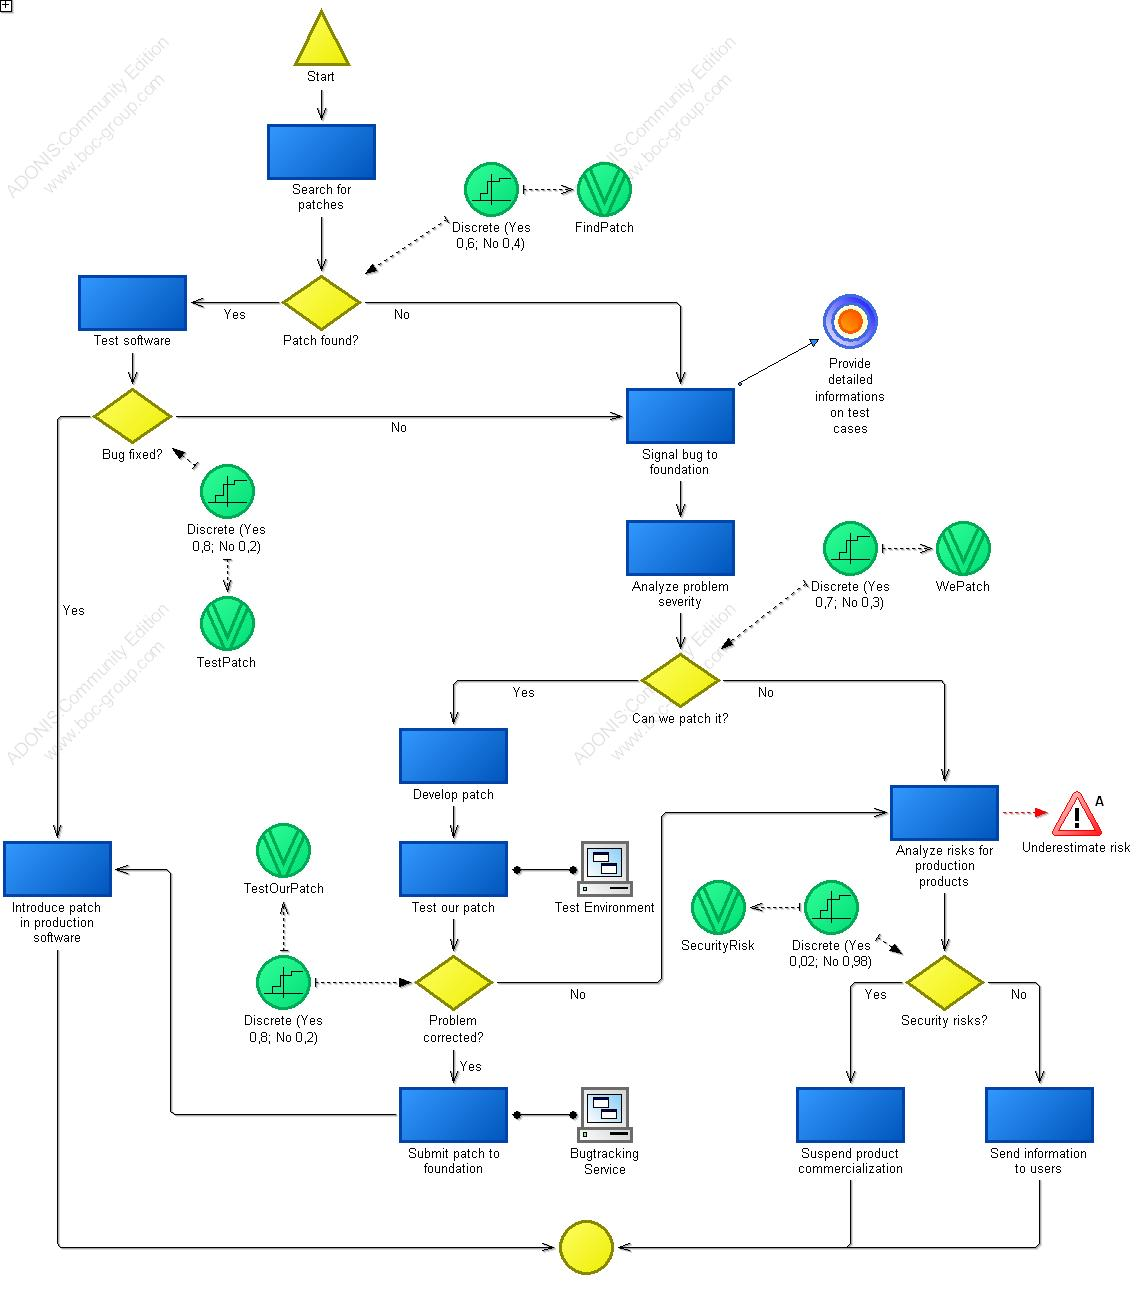
\includegraphics[scale=0.40]{assign2/adonis/imgs/coop.jpg}
\caption{Collaboration between AllSpark and OpenSource projects}
\label{2img:found_coop}
\end{centering}
\end{figure}

\subsubsection{Path Analysis}
The results of the path analysis of this process shows that the most
probable outcome of this process is that the Foundation has already
provided a working solution for the discovered problem.
The least probable paths are the ones in which neither AllSPark nor the
foundation are able to find a solution for a security related problem,
which lead to more important consequences.

\begin{table}[ht!]
\centering
\begin{tabular}{|l|l|l|l|l|}
\hline
Path&Probability&Execution&time&Costs\\
\hline
1&0,478000&00:000:04:00:00&00:000:04:00:00&151,000000\\
\hline
2&0,219000&00:010:03:55:00&00:010:03:55:00&662,000000\\
\hline
3&0,117000&00:000:01:53:00&00:000:01:53:00&31,000000\\
\hline
4&0,082000&00:010:05:25:00&00:010:05:25:00&762,000000\\
\hline
5&0,060000&00:010:01:58:00&00:010:01:58:00&631,000000\\
\hline
6&0,030000&00:000:03:23:00&00:000:03:23:00&131,000000\\
\hline
7&0,012000&00:010:03:28:00&00:010:03:28:00&731,000000\\
\hline
8&0,001000&00:000:04:13:00&00:000:04:13:00&211,000000\\
\hline
9&0,001000&00:010:04:18:00&00:010:04:18:00&811,000000\\
\hline
\end{tabular}
\end{table}

\begin{alltt}
Probability:   47,8000%
Execution time:  00:000:04:00:00
Waiting time:  00:000:00:00:00
Resting time:  00:000:00:00:00
Transport time:  00:000:00:00:00
Cycle time:  00:000:04:00:00
Costs:  151,000000

Foundations Coop 0.3 (Business process model)
========================================
Process start: Start
Activity: Search for patches
Decision: Patch found? --> FindPatch = 'Yes'
Activity: Test software
Decision: Bug fixed? --> TestPatch = 'Yes'
Activity: Introduce patch in production software
End: End-44485
\end{alltt}

\subsubsection{Capacity Analysis}
Table \ref{2tab:coop} shows how the work is divided among developers (for
the implementation part) and area manager for the analysis of product and
bug severity.

\begin{landscape}
\centering
\begin{table}
{\tiny
\begin{tabular}{|l|l|l|l|l|l|l|}
Business process&Activity&Performer&Number&Execution time&Cycle
time&Costs\\
\hline
Foundations Coop 0.3&&&&00:004:02:40:34&00:004:02:40:34&341,990000\\
\hline
&Search for patches &&1,000000&00:000:00:30:00&&1,000000\\
\hline
&&Area Manager &1,000000&00:000:00:30:00&&1,000000\\
\hline
&Test software &&0,577000&00:000:00:51:56&&57,700000\\
\hline
&&Area Manager &0,577000&00:000:00:51:56&&57,700000\\
\hline
&Introduce patch in production software &&0,774000&00:000:01:32:53&&38,700000\\
\hline
&&Area Manager &0,774000&00:000:01:32:53&&38,700000\\
\hline
&Signal bug to foundation &&0,536000&00:000:00:05:22&&0,000000\\
\hline
&&Area Manager &0,536000&00:000:00:05:22&&0,000000\\
\hline
&Analyze problem severity &&0,536000&00:000:00:32:10&&5,360000\\
\hline
&&Area Manager &0,536000&00:000:00:32:10&&5,360000\\
\hline
&Develop patch &&0,390000&00:003:09:00:00&&195,000000\\
\hline
&&Area Manager &0,390000&00:003:09:00:00&&195,000000\\
\hline
&Test our patch &&0,390000&00:000:00:01:57&&39,000000\\
\hline
&&Area Manager &0,390000&00:000:00:01:57&&39,000000\\
\hline
&Submit patch to foundation &&0,310000&00:000:00:03:06&&0,310000\\
\hline
&&Area Manager &0,310000&00:000:00:03:06&&0,310000\\
\hline
&Analyze risks for production products &&0,226000&00:000:00:00:41&&0,000000\\
\hline
&&Programmer &0,115000&00:000:00:00:21&&0,000000\\
\hline
&&Analyst &0,111000&00:000:00:00:20&&0,000000\\
\hline
&Suspend product commercialization &&0,005000&00:000:00:00:18&&0,500000\\
\hline
&&Programmer &0,002000&00:000:00:00:07&&0,200000\\
\hline
&&Analyst &0,003000&00:000:00:00:11&&0,300000\\
\hline
&Send information to users &&0,221000&00:000:00:02:13&&4,420000\\
\hline
&&Area Manager &0,221000&00:000:00:02:13&&4,420000\\
\hline
Total&&&&00:004:02:40:34&&341,990000\\
\hline
\end{tabular}
}
\caption{Capacity analysis for the process of collaboration with an
OpenSource foundation} 
\label{2tab:coop}
\end{table}
\end{landscape}




\subsection{Commercialization}
This process manages the procedure executed to evaluate if a research
project is ready to be actually converted in a effective product.
Is important to notice that this decision depends on on the market data and
on the need of the customer.

It can be the case that a project is not ready to be commercialized, or,
instead, the project is ready but the market and the customers don't yet
need this new product, at this moment.

If this is the case, is necessary to delay the commercialization of the
product waiting for a moment in which it can be more appreciated.
This process is described in figure \ref{2img:commerce}

\begin{figure}[!ht]
\begin{centering}
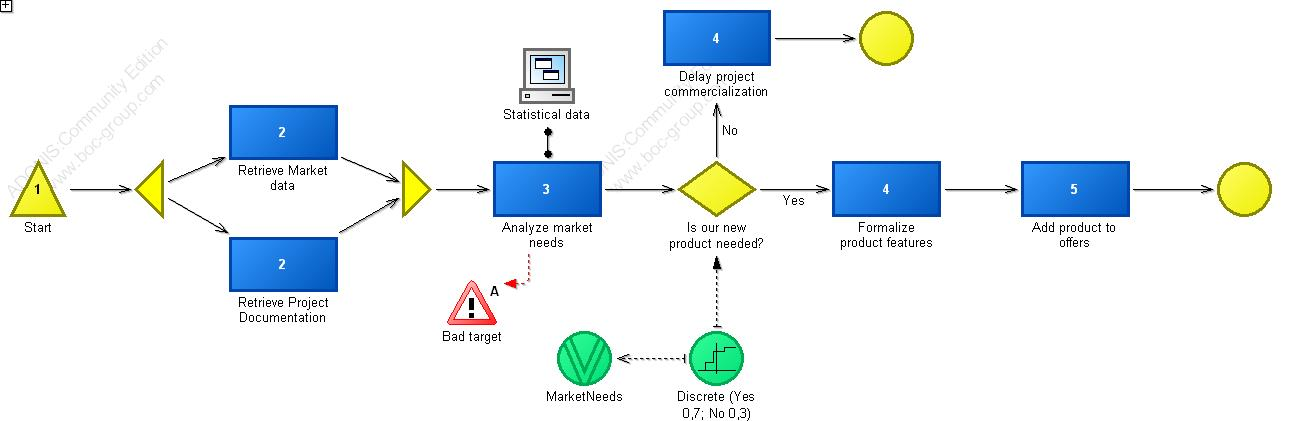
\includegraphics[scale=0.45,angle=90]{assign2/adonis/imgs/commercialize.jpg}
\caption{Commercialization of a research project}
\label{2img:commerce}
\end{centering}
\end{figure}

\subsubsection{Path Analysis}
The analysis of the possible paths shows that the most probable, with 71\%
pf probability, id that a project is accepted as a new product.
The other one, which leads to the delay of the commercialization of the
product, has a probability of 30\%.

\begin{table}[ht!]
\centering
\begin{tabular}{|l|l|l|l|l|}
Path&Probability&Execution&time&Costs\\
\hline
1&0,686000&00:000:00:46:00&00:000:00:43:00&110,400000\\
\hline
2&0,314000&00:000:00:28:00&00:000:00:25:00&5,400000\\
\hline
\end{tabular}
\end{table}


\begin{alltt}
Probability:   71,7000%
Execution time:  00:000:00:46:00
Waiting time:  00:000:00:00:00
Resting time:  00:000:00:00:00
Transport time:  00:000:00:00:00
Cycle time:  00:000:00:43:00
Costs:  110,400000

Commercializing 0.3 (Business process model)
========================================
Process start: Start
Parallelity: Parallelity-41066
    *
    Activity: Retrieve Project Documentation
    *
    Activity: Retrieve Market data
Merging: Merging-41072
Activity: Analyze market needs
Decision: Is our new product needed? --> MarketNeeds = 'Yes'
Activity: Formalize product features
Activity: Add product to offers
End: End-41103
\end{alltt}



\subsubsection{Capacity Analysis}
Table \ref{2tab:commerc} shows the capacity analysis for the roles involved in
the commercialization of a research project.
\begin{landscape}
\centering
\begin{table}
{\tiny
\begin{tabular}{|l|l|l|l|l|l|l|}
Business process&Activity&Performer&Number&Execution time&Cycle
time&Costs\\
\hline
Commercializing 0.3&&&&00:000:00:40:08&00:000:00:37:08&76,170000\\
\hline
&Retrieve Project Documentation &&1,000000&00:000:00:03:00&&0,200000\\
\hline
&&Area Manager &1,000000&00:000:00:03:00&&0,200000\\
\hline
&Retrieve Market data &&1,000000&00:000:00:03:00&&0,200000\\
\hline
&&Area Manager &1,000000&00:000:00:03:00&&0,200000\\
\hline
&Analyze market needs &&1,000000&00:000:00:20:00&&5,000000\\
\hline
&&Area Manager &1,000000&00:000:00:20:00&&5,000000\\
\hline
&Formalize product features &&0,674000&00:000:00:10:07&&3,370000\\
\hline
&&Area Manager &0,674000&00:000:00:10:07&&3,370000\\
\hline
&Add product to offers &&0,674000&00:000:00:03:22&&67,400000\\
\hline
&&Programmer &0,340000&00:000:00:01:42&&34,000000\\
\hline
&&Analyst &0,334000&00:000:00:01:40&&33,400000\\
\hline
&Delay project commercialization &&0,326000&00:000:00:00:39&&0,000000\\
\hline
&&Area Manager &0,326000&00:000:00:00:39&&0,000000\\
\hline
\end{tabular}
}
\caption{Capacity analysis for the process of commercialization of a
research project}
\label{2tab:commerc}
\end{table}
\end{landscape}



